\documentclass[11pt]{article}

\usepackage[margin=1in]{geometry}
\usepackage{graphicx}
\usepackage{hyperref}
\usepackage{booktabs}
\usepackage{enumitem}
\usepackage{xcolor}
\usepackage{mdframed}
\usepackage{array}
\usepackage{caption}

\hypersetup{
    colorlinks=true,
    linkcolor=blue,
    filecolor=magenta,      
    urlcolor=blue,
    pdftitle={Assignment 1: Opinion Network Formation},
}

\title{\textbf{Assignment 1: Opinion Network Formation}}
\author{DPCN Course — 2026}
\date{20 September 2026}

\begin{document}

\maketitle

\section*{Team Name}
\textbf{clankers}
\vspace{0.5cm}\hrule\vspace{0.5cm}

\section*{GitHub Link to Your Code}
\textbf{Repository:} \href{https://github.com/DPCN-M26/Opinion-Network-Formation-A1.git}{https://github.com/DPCN-M26/Opinion-Network-Formation-A1.git}

\begin{mdframed}[backgroundcolor=black!5, linecolor=black!10]
\textbf{Note:} The repository contains: \texttt{Opinion\_Network\_Analysis.ipynb} (the full annotated Jupyter Notebook) and \texttt{dataset.csv} (the survey data). All plots are generated reproducibly by running the notebook.
\end{mdframed}
\vspace{0.5cm}\hrule\vspace{0.5cm}

\section{Dataset Documentation}
The dataset contains survey responses from \textbf{96 students}, each answering \textbf{60 questions} (15 per topic) on the following four categories:

\begin{center}
\begin{tabular}{@{}llc@{}}
\toprule
\textbf{Code} & \textbf{Topic} & \textbf{No. of Questions} \\ \midrule
T01--T15 & Technology \& Artificial Intelligence & 15 \\
E01--E15 & Education \& Academia & 15 \\
S01--S15 & Society \& Ethics & 15 \\
V01--V15 & Environment \& Sustainability & 15 \\ \bottomrule
\end{tabular}
\end{center}

Each question was answered on a \textbf{5-point Likert scale}: Strongly Disagree, Disagree, Neutral, Agree, Strongly Agree. A small number of responses were marked "No Comments."

\subsection*{Preparation \& Encoding}
\begin{enumerate}
    \item \textbf{Numerical mapping:} We mapped responses to signed integers to capture opinion direction: Strongly Disagree $\rightarrow -2$, Disagree $\rightarrow -1$, Neutral $\rightarrow 0$, Agree $\rightarrow +1$, Strongly Agree $\rightarrow +2$. "No Comments" was mapped to $0$ (treated as Neutral/abstention).
    \item \textbf{Baseline sentiment:} The average scores show that the class held \textit{consistently positive} views across all topics:
    \begin{itemize}
        \item Technology: \textbf{+0.928} \quad|\quad Education: \textbf{+0.819}
        \item Society: \textbf{+1.151} \quad|\quad Environment: \textbf{+1.226}
    \end{itemize}
    Environment and Society questions received the strongest agreement overall, while Education responses showed the most nuanced spread.
    \item \textbf{Positive-shifting for TF-IDF:} To apply TF-IDF (which requires non-negative counts), the values were shifted from $[-2, +2]$ to $[1, 5]$, preserving relative magnitudes.
\end{enumerate}

\section{Pipeline Followed}
Our pipeline is innovative because it goes \textbf{beyond standard cosine similarity}. We use three complementary approaches that are central to the theme of this course: \textit{network construction}, \textit{static network analysis}, and \textit{dynamical processes on networks}.

\subsection{Step 1: TF-IDF Weighted Similarity Network}
Instead of treating all shared opinions equally, we applied \textbf{Term Frequency-Inverse Document Frequency (TF-IDF)} — borrowing from Natural Language Processing — where each student is a "document" and each survey response is a "term." TF-IDF assigns a lower weight to responses that the \textit{majority} of the class agreed on, and a \textit{higher weight} to rare, distinguishing opinions. This ensures that the resulting edge weights reflect \textbf{genuine ideological proximity}. After computing pairwise cosine similarity, we applied a \textbf{70th percentile threshold} to retain only the strongest 30\% of potential connections.

\subsection{Step 2: Community Detection (Louvain Algorithm)}
We applied the \textbf{Louvain algorithm} (modularity-maximization) to detect communities within the TF-IDF network. This algorithm partitions nodes into communities that maximize intra-community edge density relative to chance (measured by the \textbf{modularity score Q}).

\subsection{Step 3: Multiplex Network Analysis (4-Layer)}
We constructed a \textbf{4-layer multiplex network} — one layer each for Technology, Education, Society, and Environment — to study whether opinions are correlated \textit{across topics}. A high Jaccard edge-overlap between two layers means students who agree ideologically on one topic also tend to agree on another.

\subsection{Step 4: Opinion Dynamics — Deffuant Bounded Confidence Model}
We simulated how classroom consensus (or fragmentation) would emerge if students interacted and influenced each other using the \textbf{Deffuant model}:
\begin{itemize}
    \item Initial opinion state = average score across all 60 questions.
    \item At each time step, a random connected pair $(u, v)$ is selected. If their opinions differ by less than the confidence threshold $\varepsilon = 0.5$, they update toward each other: $x_u \leftarrow x_u + \mu(x_v - x_u)$, with convergence rate $\mu = 0.3$.
    \item The simulation runs for \textbf{8,000 steps} on the TF-IDF network.
    \item A GIF animation (\texttt{opinion\_dynamics.gif}) visually shows how node colours (red=disagree, green=agree) shift across the network over time.
\end{itemize}

\section{Analysis and Visualizations}

\subsection{Network Metrics Summary}
\begin{center}
\begin{tabular}{@{}lr@{}}
\toprule
\textbf{Metric} & \textbf{Value} \\ \midrule
Nodes (students) & 96 \\
Edges (strong ideological links) & 1,368 \\
Network Density & 0.30 \\
Average Degree & 28.50 \\
Average Clustering Coefficient & 0.678 \\
Connected Components & 11 \\
Communities (Louvain) & 13 \\
Modularity (Q) & 0.106 \\ \bottomrule
\end{tabular}
\end{center}

The network has a \textbf{density of 0.30} (moderately dense) and a high \textbf{average clustering coefficient of 0.678} (strong clique structure). The \textbf{11 connected components} reveal that a small number of students are ideological outliers who share strong connections with no one in the main cluster.

\subsection{Centrality: Opinion Influencers}
We compute two complementary centrality measures:

\textbf{Degree Centrality} (broadest connectors):
\begin{center}
\begin{tabular}{@{}clc@{}}
\toprule
\textbf{Rank} & \textbf{Student} & \textbf{Degree Centrality} \\ \midrule
1 & Student 44 & 0.7368 \\
2 & Student 60 & 0.7368 \\
3 & Student 68 & 0.7368 \\
4 & Student 73 & 0.7368 \\
5 & Student 78 & 0.7368 \\ \bottomrule
\end{tabular}
\end{center}

\textbf{Betweenness Centrality} (opinion brokers bridging communities):
\begin{center}
\begin{tabular}{@{}clc@{}}
\toprule
\textbf{Rank} & \textbf{Student} & \textbf{Betweenness Centrality} \\ \midrule
1 & Student 67 & 0.0533 \\
2 & Student 14 & 0.0249 \\
3 & Student 77 & 0.0242 \\
4 & Student 97 & 0.0237 \\
5 & Student 41 & 0.0235 \\ \bottomrule
\end{tabular}
\end{center}
\textbf{Student 67} is the most critical structural actor: the key ideological \textbf{broker} between communities.

\newpage
\subsection{Figure 1: TF-IDF Opinion Network}
\begin{figure}[h]
    \centering
    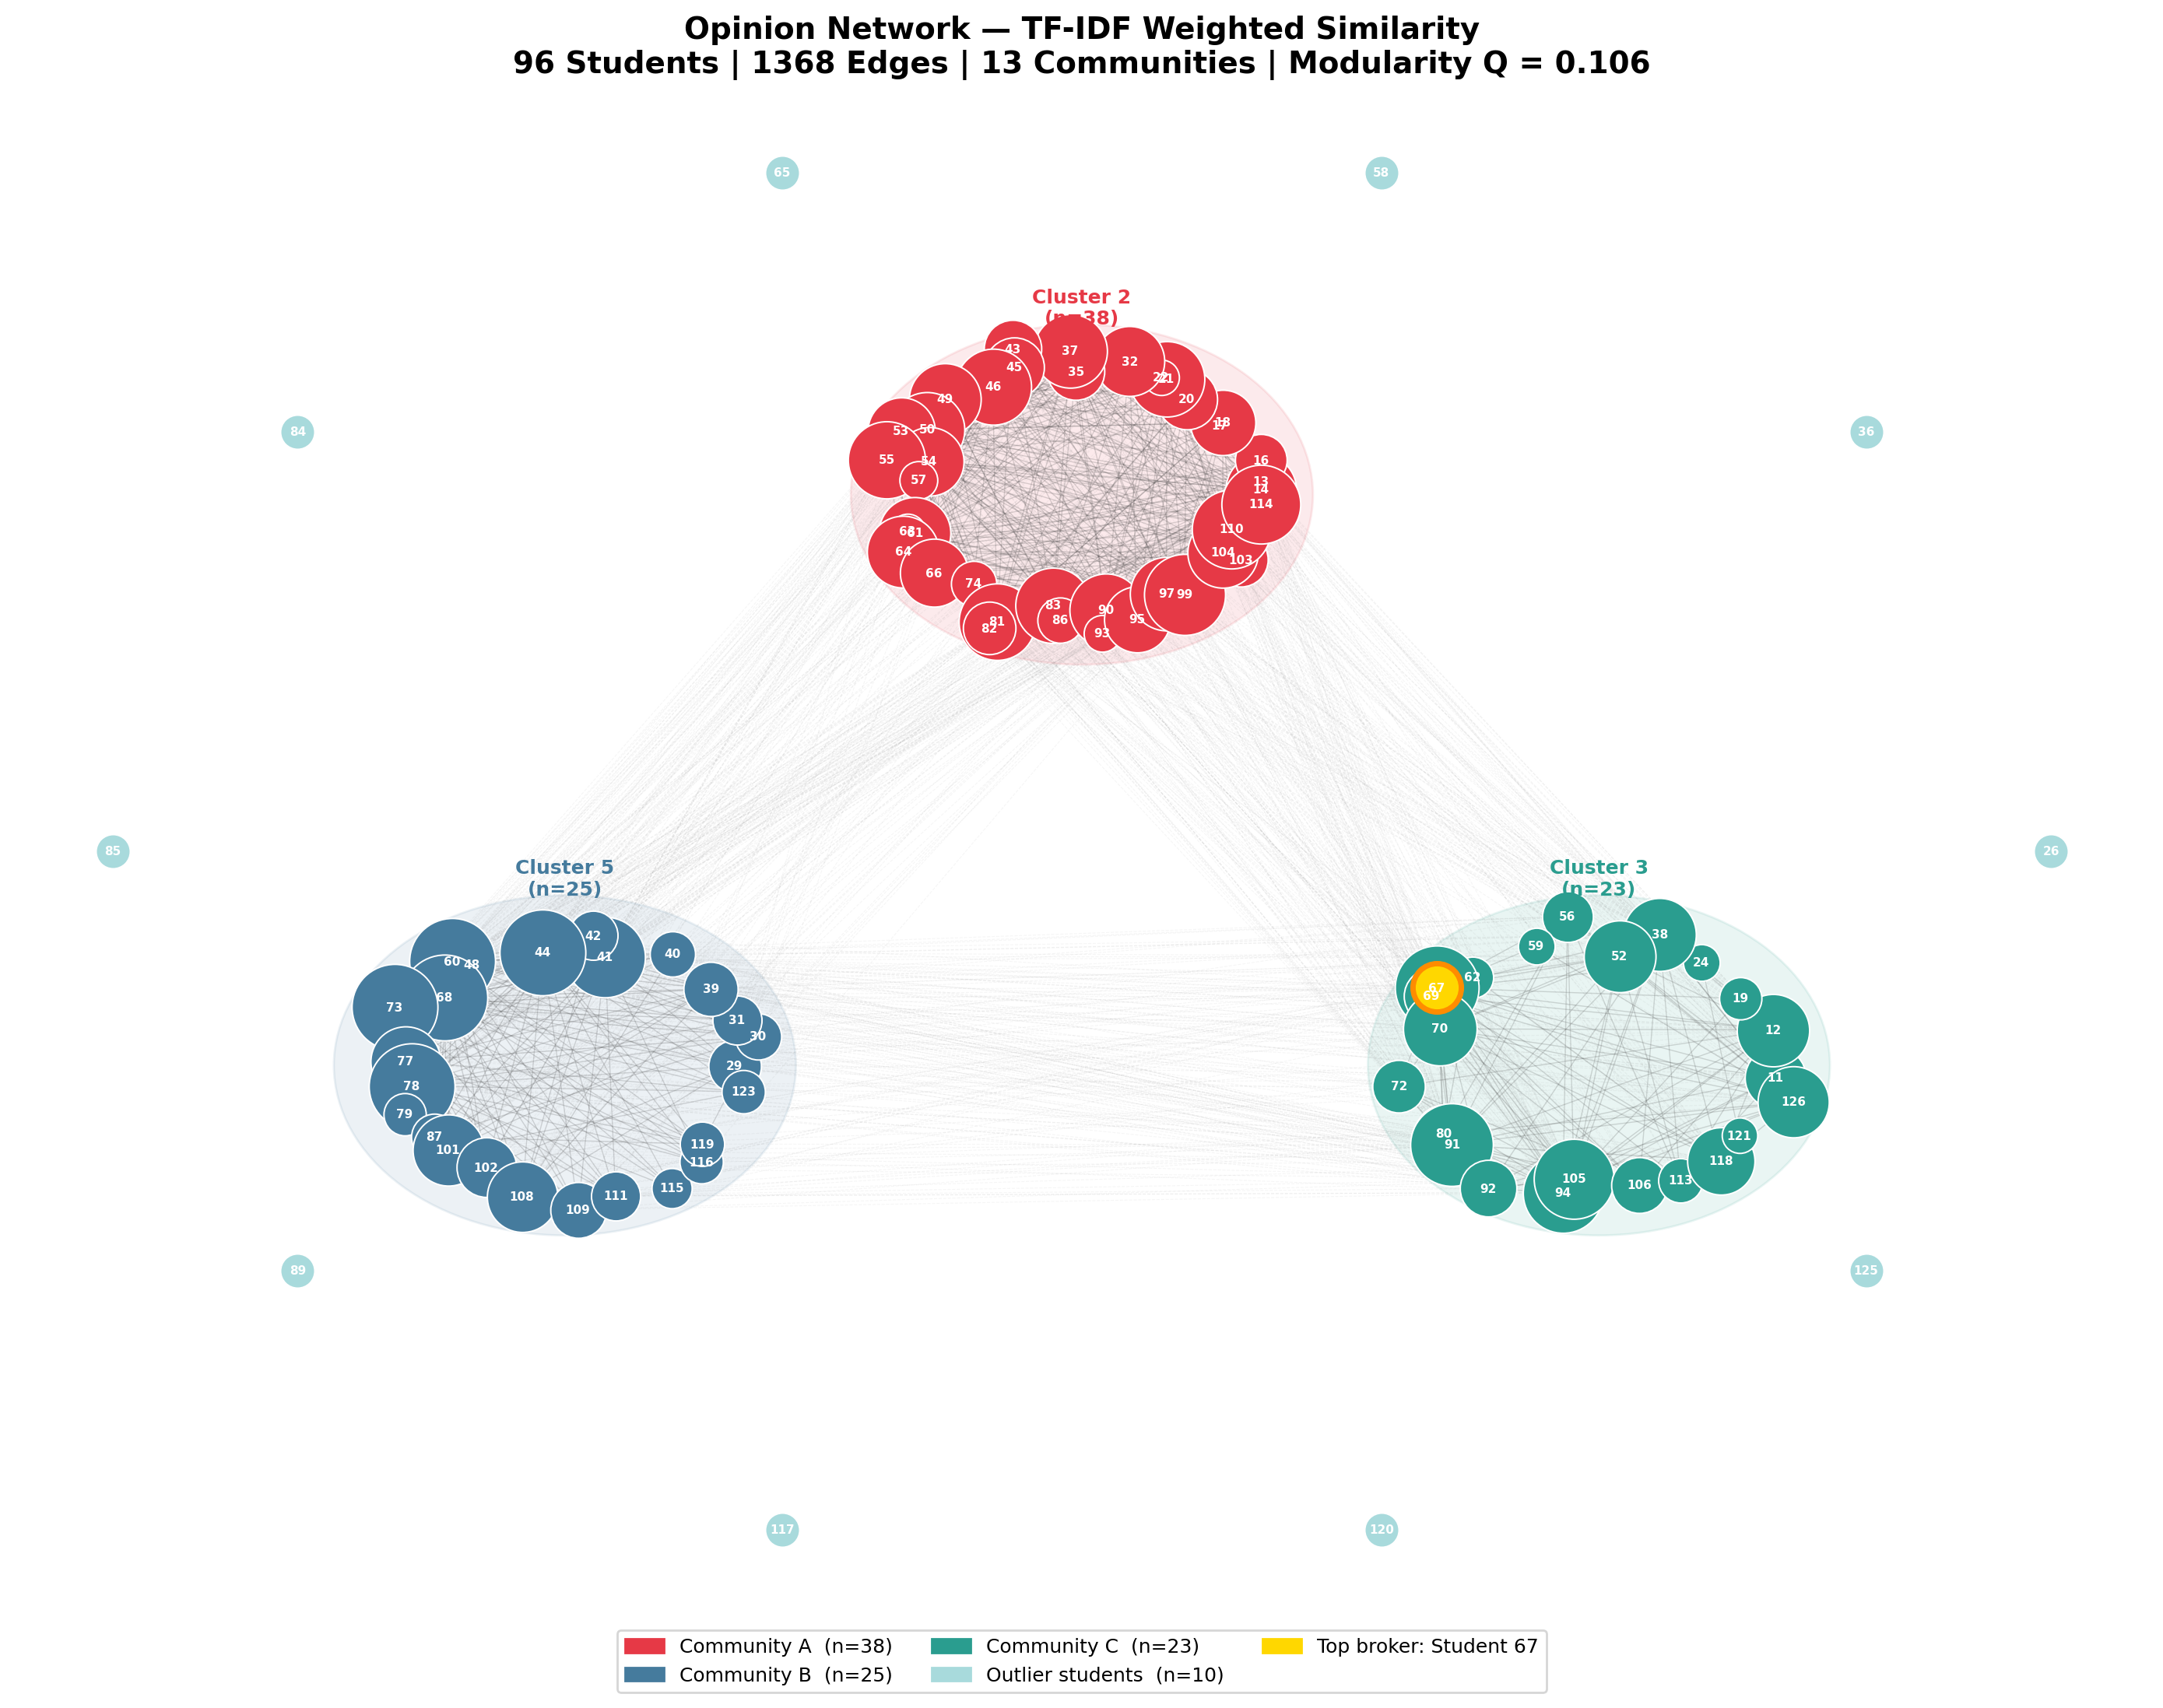
\includegraphics[width=\textwidth]{opinion_network.png}
    \caption{The Opinion Network arranged using a community-aware layout. The three main clusters are placed at the vertices of a triangle. Node size scales with degree centrality. The gold-ringed node is \textbf{Student 67} (highest betweenness centrality). The 10 outlier students (cyan) float around the periphery.}
\end{figure}

The network reveals three dominant ideological clusters (n=38 red, n=25 blue, n=23 teal) accounting for \textbf{86\% of the class}. This confirms the class is \textbf{not polarized} (no two opposing camps), but differentiates into three ideologically nuanced groups with significant common ground.

\subsection{Figure 2: Topic-Level Average Scores}
\begin{figure}[h]
    \centering
    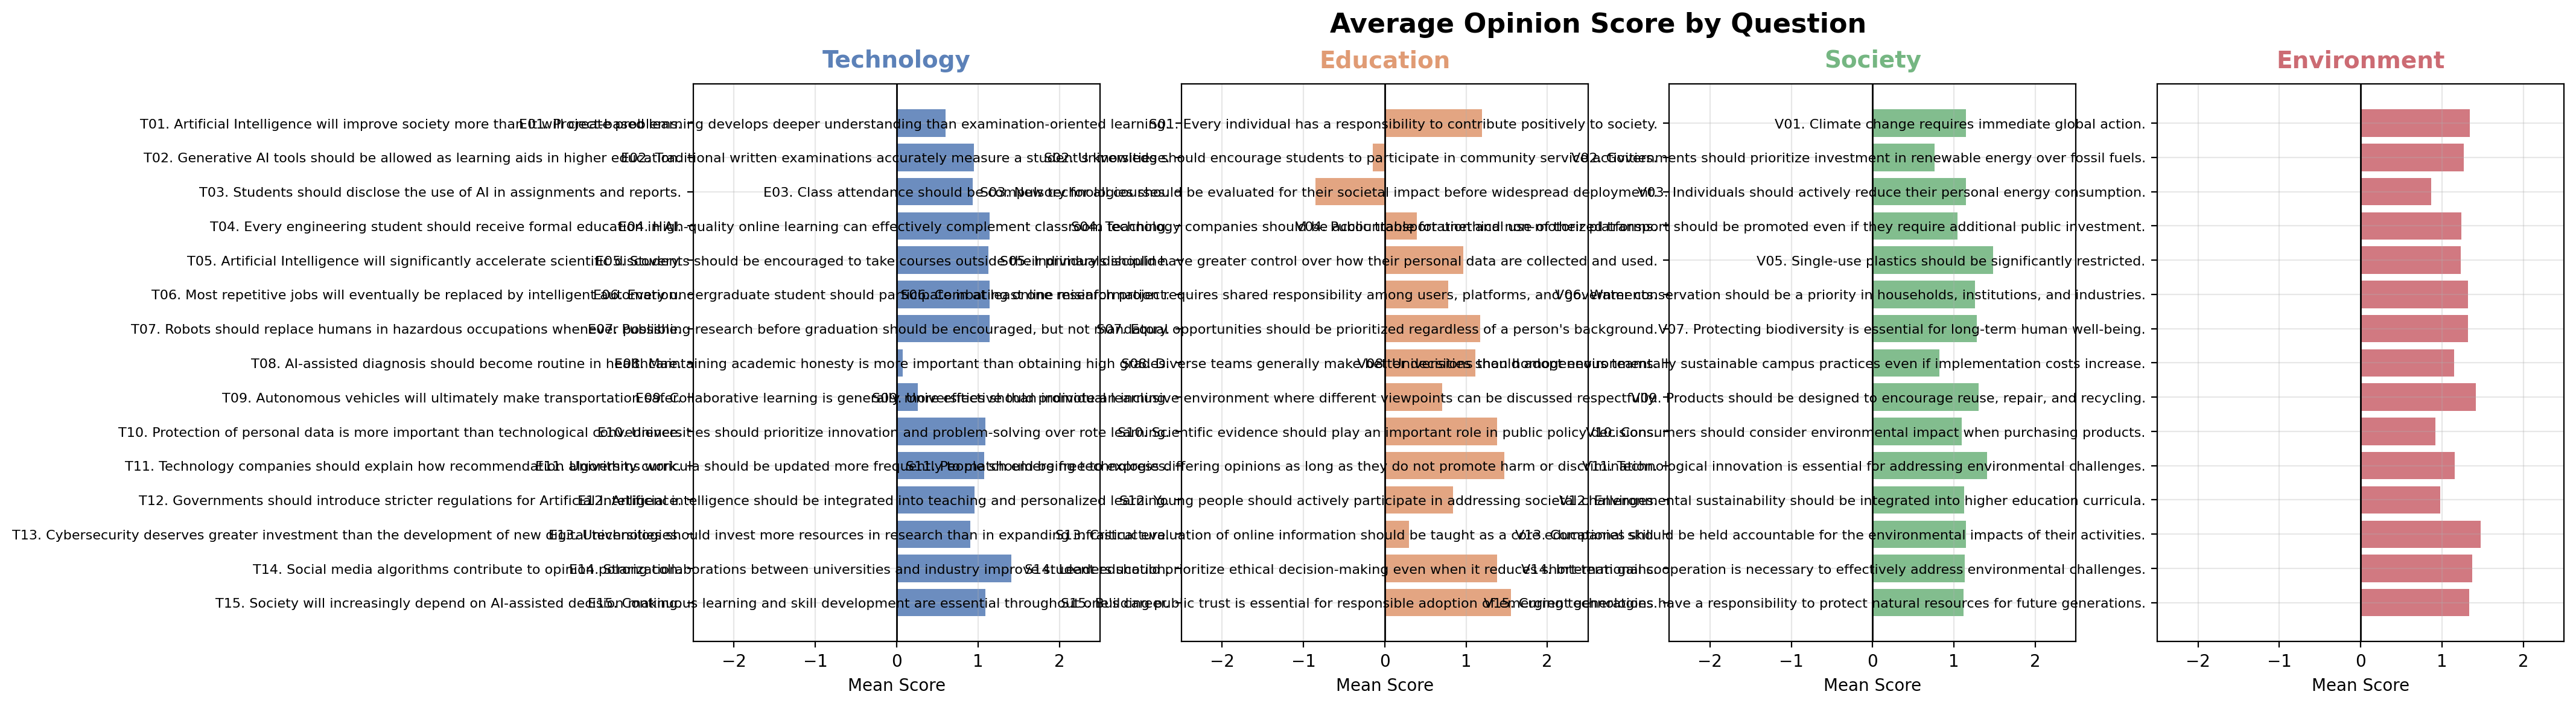
\includegraphics[width=0.9\textwidth]{topic_scores.png}
    \caption{Mean response score ($-2$ to $+2$) per question, broken down by the four survey topics.}
\end{figure}
Almost all bars lean positive. Within Technology, questions about AI replacing jobs (T06) and government regulation (T12) show the lowest scores. Within Education, opposition to mandatory attendance (E03) and skepticism about traditional exams (E02) stand out.

\subsection{Figure 3: Multiplex Edge Overlap}
\begin{figure}[h]
    \centering
    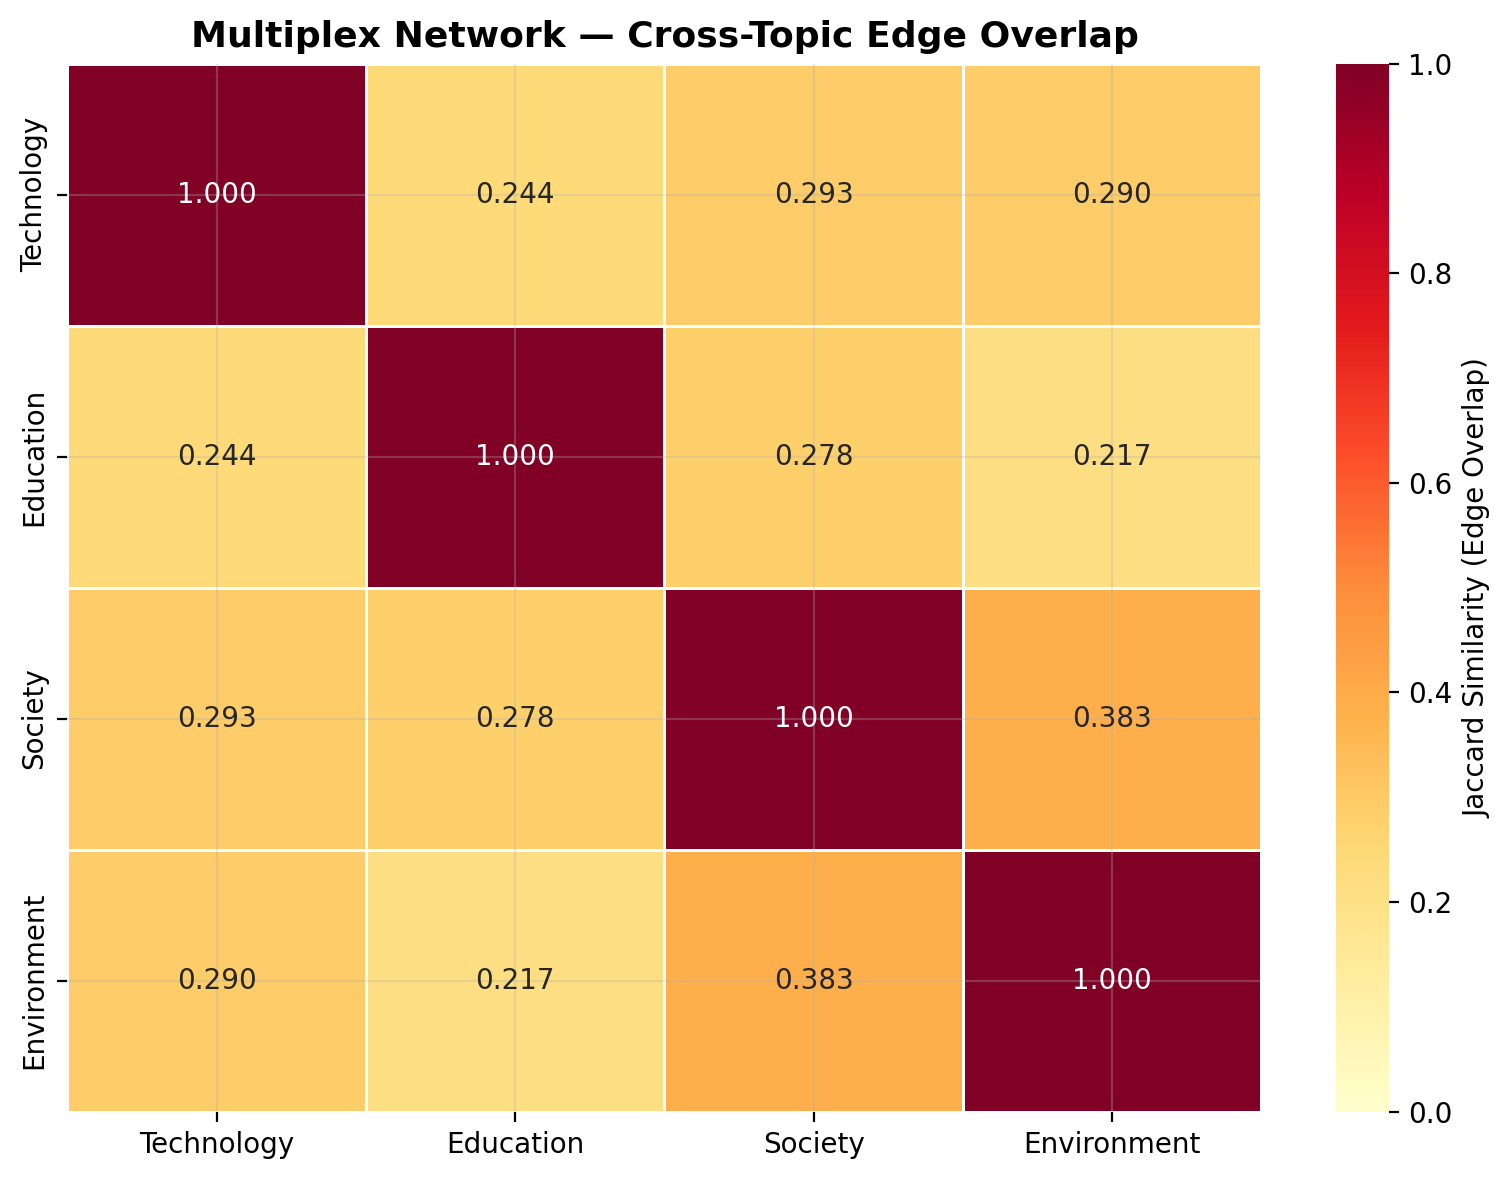
\includegraphics[width=0.7\textwidth]{multiplex_overlap.png}
    \caption{Jaccard similarity of edge sets between the four topic-specific network layers.}
\end{figure}
The highest overlap is between \textbf{Society and Environment (0.383)}. The weakest connection is between \textbf{Education and Environment (0.217)}, suggesting that educational philosophy is the most independent of all four topic domains.

\subsection{Figure 4: Opinion Dynamics (Deffuant Model)}
\begin{figure}[h]
    \centering
    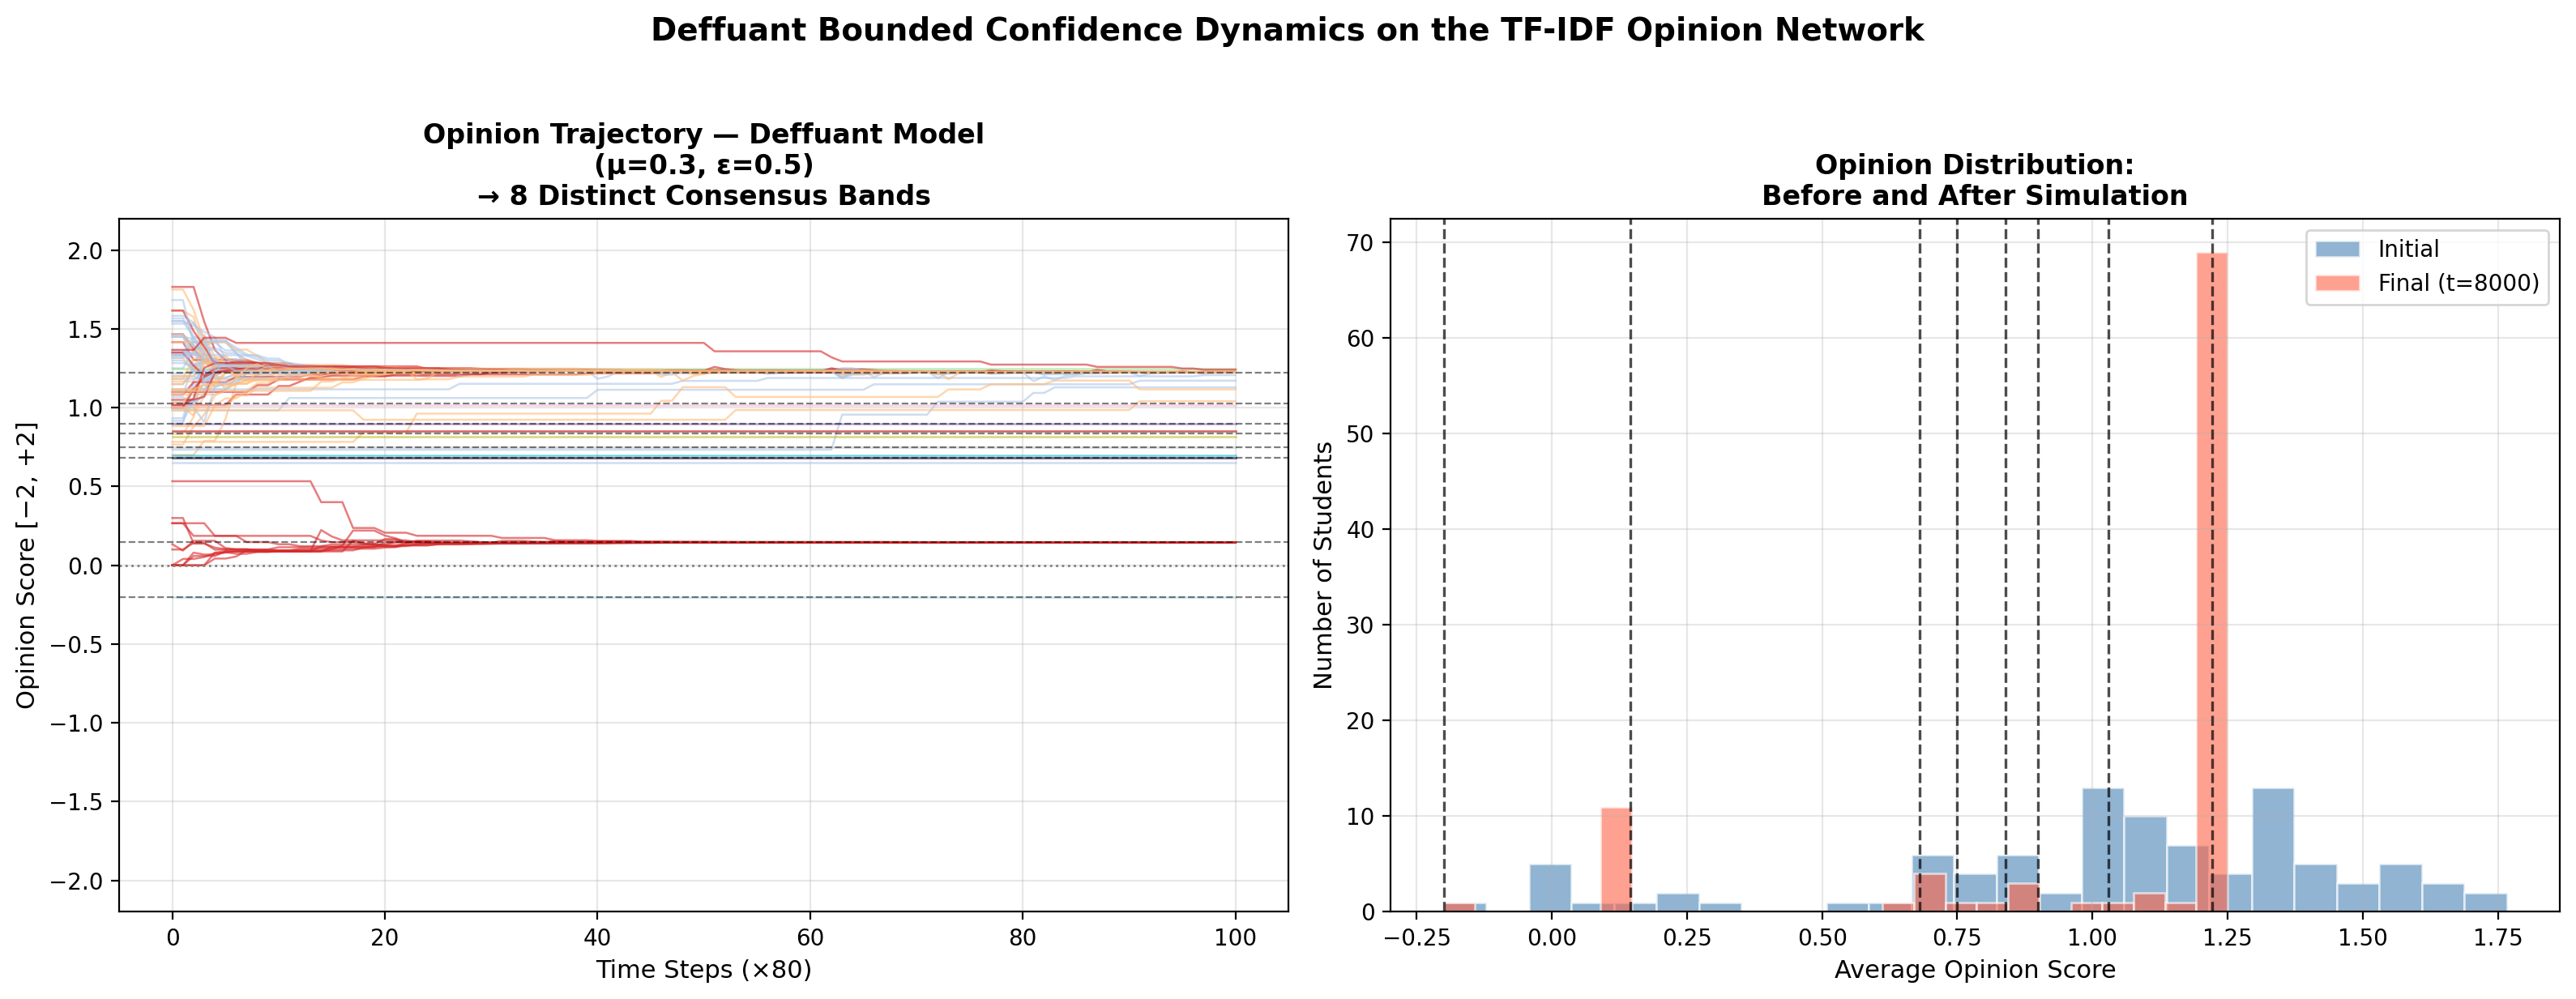
\includegraphics[width=\textwidth]{opinion_dynamics.png}
    \caption{(Left): Opinion trajectory for each student over 8,000 simulation steps. (Right): Histogram showing the dramatic narrowing of the initial spread into 8 distinct attractor bands.}
\end{figure}
\begin{itemize}
    \item \textbf{Initial distribution:} Mean = $+1.03$, spread widely across $[-0.2, +1.8]$.
    \item \textbf{Final distribution:} Mean = $+1.03$, Std = $0.376$, fragmented into \textbf{8 distinct consensus bands}.
    \item The system does \textbf{not} converge to a single consensus. Instead, it freezes into \textbf{8 attractor states} (echo chambers), the largest containing 72 students. The 10 outlier students retain their initial opinions, as they have no network connections — a direct demonstration that \textbf{topology constrains dynamics}.
\end{itemize}

\section{Results and Discussion}
The analysis reveals several key insights:
\begin{enumerate}
    \item \textbf{The class is not polarized; it is differentiated into a nuanced consensus.} Three large clusters account for 86\% of students.
    \item \textbf{Opinion alignment is topic-specific, not global.} The multiplex analysis proves that someone who shares your views on Technology is not necessarily aligned with you on Education.
    \item \textbf{The most structurally important student is not the most popular one.} Student 67 has the highest \textit{betweenness} centrality, while others have the highest \textit{degree} centrality.
    \item \textbf{Bounded confidence creates echo chambers, not consensus.} The Deffuant simulation shows the system fragmenting into 8 final attractor states.
    \item \textbf{Network topology directly controls which dynamics are possible.} The isolated outlier students never change their opinions because they have no edges in the network.
\end{enumerate}

\section{Individual Contribution}
\begin{center}
\begin{tabular}{@{}p{3.5cm} p{11.5cm}@{}}
\toprule
\textbf{Team Member} & \textbf{Tasks} \\ \midrule
\textbf{Ch shreyash} & End-to-end pipeline design, data preprocessing, network construction (TF-IDF), community detection, multiplex analysis, Deffuant model simulation, visualization programming, and report drafting. \\
\textbf{Vansh Motwani} & Codebase review, verification of analysis methodology, parameter tuning validation, and peer-review of the final report. \\ \bottomrule
\end{tabular}
\end{center}

\end{document}
